\documentclass[twoside,10.5pt]{article}


\usepackage{jmlr2e}
\usepackage{graphicx}
\usepackage{subcaption}
\captionsetup{compatibility=false}

\newcommand{\dataset}{{\cal D}}
\newcommand{\fracpartial}[2]{\frac{\partial #1}{\partial  #2}}

% Heading arguments are {volume}{year}{pages}{date submitted}{date published}{paper id}{author-full-names}
\newcommand{\N}{\mathbb{N}}
\newcommand{\Z}{\mathbb{Z}}
\newcommand{\I}{\mathrm{I}}
\newcommand{\E}{\mathrm{E}}
\newcommand{\Var}{\mathrm{Var}}
\newcommand{\argmax}{arg\,max}
\newcommand{\argmin}{arg\,min}
\newcommand{\arginf}{arg\,inf}
\newtheorem{claim}{Claim}[section]




% Short headings should be running head and authors last names

\ShortHeadings{Final Project - EECS504}{Tianchen Zhao, Julio Soldevilla}
\firstpageno{1}

\begin{document}

\title{Image Segmentation using Markov Random Field Model}

\author{\name Tianchen Zhao \email ericolon@umich.edu \\
       \addr Department of Mathematics\\
       University of Michigan\\
       Ann Arbor, MI 48104, USA       \AND
       \name Julio Soldevilla \email jsolde@umich.edu \\
       \addr Department of Mathematics\\
       University of Michigan\\
       Ann Arbor, MI 48104, USA}

\editor{Julio Soldevilla, Tianchen Zhao}

\maketitle

%\begin{abstract}
%\end{abstract}
%
%\begin{keywords}
%\end{keywords}

\section{Introduction}
We are interested in the image segmentation problem from a pixel labelling approach: each pixel of an image is assigned to a label $z \in \mathcal{Z}$, where $\mathcal{Z}$ is the class of labels available. The label assignment is achieved by using a parametrized probablistic model.

In real images, neighboring pixels usually have similar features. One reasonable model that could capture this contextual constraint is the Markov Random Field(MRF) model, decribed as follows:
\begin{definition}
Given a $M \times N$ image $I$ and a neighborhood system $\eta$, it's a MRF if for every pixel $I_{ij}$,
\begin{equation}
P(I_{ij}=x_{ij}|I_{kl}=x_{kl}, (k,l) \neq (i,j)) = P(I_{ij}=x_{ij}|I_{kl}=x_{kl}, (k,l) \in \eta(i,j)),
\end{equation}
and $P(I_{ij}=x_{ij})>0$.
\end{definition}
According to Hammersley-Clifford Theorem, an image modelled by $MRF$ is Gibbs distributed, which is of the form:
\begin{equation} \label{eq:1}
P(I=x;\theta) = \frac{1}{\beta} e^{-U(x)},
\end{equation}
where $\beta$ is the partition function and $U$ is the energy function encoding the prior knowledge of the image, enforcing the smoothness condition on the segmentation(\citet{Brgisser2013}).

Also assume that given a pixel value $x$, the conditional probability for the label is given by:
\begin{equation} \label{eq:2}
P(Z_{ij}=z|I=x; \theta) = \frac{1}{(2\pi \sigma(z)^2)^{MN/2}}e^{\frac{-||x-\mu(z)||^2}{2\sigma(z)^2}},
\end{equation}
where $\sigma$ and $\mu$ are the variance and mean dependent on the label $z$.

From (\ref{eq:1}) and (\ref{eq:2}), we can compute the objective function:
\begin{equation}
P(Z_{ij}=z|I = x; \theta) = P(I=x;\theta) P(Z_{ij}=z|I=x; \theta).
\end{equation}

\section{Related work and our approach}

Image segmentation is a classic problem in computer vision. Several researchers have tried to solve this problem, some of the approaches we studied in class were the variational methods, like the Mumford Shah model or graph methods, like min-cut/max flow algorithms for background and foreground segmentation using MRF. Furthermore, we studied thoroughly histogram based methods that segment images based on the intensity of the color of the picture. In class, we touched on Markov Random Fields methods (MRF) so for this project we decided to explore more of this segmentation method. In Markov Random Fields, in supervised methods, we end up having the problem of minimizing a nonconvex function and the issue reduces to finding a suitable way to optimize such a problem, without just staying in a local optimum. A  popular approach for this problem was to do simulated annealing or to use metropolis dynamics for energy minimization. In the unsupervised case, we decided to focus on using the tabu search optimization method to find the segmentation of our image. In the unsupervised case we implemented the EM algorithm to find the segmentation. 

To solve the problem of image segmentation we followed two approaches: one supervised setting using Tabu Search (following Patra and Nanda (2007)) and one unsupervised setting using te EM algorithm to obtain the optimal mean and labels.

\subsection{HTS search}
As introduced by \citet{Patra:2007:ISU:1335117.1335489}, in the supervised learning setting, we are given a class of images of interest $\mathcal{I}$ and we assume we know the number of regions and the parameters $\theta = [\beta,\mu,\sigma^2]$. The final objective is to find labels $\hat{z}_{i,j}$ such that 
\begin{equation} \label{eq:3}
\hat{z_{ij}}=\argmax_{z \in \mathcal{Z}} P(Z_{ij}=z|J; \hat{\theta}).
\end{equation}

To find the segmentation we take one training image $I \in \mathcal{I}$ with label $Z$, then apply the optimization algorithm Hybrid Tabu Search(HTS) described in  \citet{Patra:2007:ISU:1335117.1335489} to obtain the optimal labelling that maximizes (5). Using a Bayesian approach, this implies using the Tabu Search algorithm to minimize the energy function given by 
\begin{equation}
    U(x,\theta) = \log(\frac{1}{\sqrt{2\pi} \sigma}) - \frac{x_{i.j} - \mu}{2\sigma^2} + V_{c_2}(i,j)
\end{equation} 

where the first term in equation 6 is the energy for the singleton cliques centered at certain pixel and $V_{c_2}(i.j)$ is the energy for doubleton cliques located at certain pixels and 

\[ V_{c_2}(i,j) = \left\{
\begin{array}{ll}
      -\beta & label(x_{i,j}) = label(x_{i+1,j}) \\
      \beta & label(x_{i,j}) \neq label(x_{i-1,j}) \\
\end{array} 
\right. \]

In this approach, we based the algorithm we created by following suggestions from \citet{Patra:2007:ISU:1335117.1335489} for the Tabu search part and suggestions from the paper "Bayesian Image Classification Using Markov Random Fields" by Zoltan Kato et. al. (the bibtex reference for this paper is not working)\footnote{http://www.inf.u-szeged.hu/~kato/papers/ivc96.pdf}. 

\subsection{EM}
We also consider the unsupervised learning setting where the mean and variance are treated as the latent variable of a given image. In this setting the EM algorithm can be applied to update the label and the mean alternatively throughout the training process. To be more precise, given the current labelled image $I$, at each iteration of the training process, we first compute the the mean and variance for each label $z \in \mathcal{Z}$ as:
\begin{equation}
\mu(z) = \frac{1}{|Z_{ij}=z|} \sum_{Z_{ij}=z} I_{ij}, \sigma(z)^2 = \frac{1}{|Z_{ij}=z|} \sum_{Z_{ij}=z}  (I_{ij}-\mu(z))^2.
\end{equation}
Then (\ref{eq:2}) is updated to a new objective function, which is a strictly convex problem and the solution can be found explicitly using differential calculus as follows:
\begin{equation}
P(Z_{ij}=z|I = x; \theta) \sim \prod_{z \in \mathcal{Z}}N(\mu(z), \sigma(z)) e^{-U(a)}
\end{equation}
The value with the highest probability is assigned to $Z_{ij}$. Part of the training process and the basic set up are done by using the nipy package. We modified the code upon it. In particular, we enforce the regularized boundary condition by addtion the regularizer to the original potential function $U$.

\section{Results and discussion}
\subsection{HTS search}
As can be seen from Figure~\ref{fig:resultsAlgorithms}, the Hybrid Tabu search algorithm used perturbs the image on every iteration to try to find the global optimum solution and not be stuck in local solutions. Because of this, even after 10 iterations, the outputs of the algorithm still show a significant amount of noise. The remnant amount of noise will be tied to the original $\sigma$ inputed by th user. Nevertheless, we can clearly see different regions corresponding to different segments of the picture. This is particularly obvious for the images 1b in Figure~\ref{fig:resultsAlgorithms}, in the last two images. In these two images, we can clearly distinguish the regions that form the original picture. We have a small issue in the second image on Figure~\ref{fig:resultsAlgorithms}b, where we are losing some of the geometrical figures because the color of the lost triangles is too bright and and so when converted to gray scale images, this colors are too close to being the same as the background color. Also, in the third picture of Figure~\ref{fig:resultsAlgorithms}b, we don't see a very clear distinction between the circle figure and the chess background, even though in the original image these figures clearly have different intensities. Again, this could happen because of the noise inherent in the Tabu search algorithm, affecting too much the white circle.

One further drawback from this Tabu Search algorithm is that the computation of the energy of the image is very slow. Because of this, larger pictures (like the horse picture shown below) take too long to run and so we weren't able to get results for that image. In general, runnig 10 iterations of the algorithm for a suitable size image ($600 \times 700$ pixels) takes around 35 minutes.

\subsection{EM}

\begin{figure*}[t!]
\label{fg:1}
%\begin{center}
\centering
    \begin{subfigure}[b]{0.45\textwidth}
        \centering
        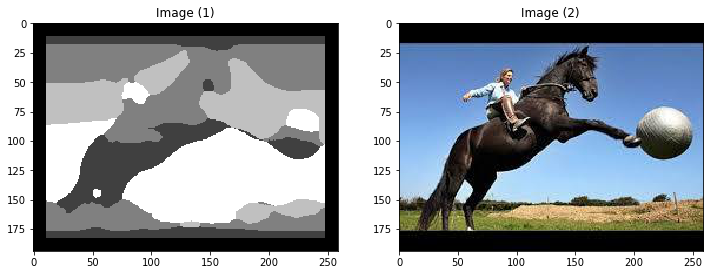
\includegraphics[width=.95\linewidth]{horse_result.png}
        %\\[\baselineskip]% adds vertical line spacing
        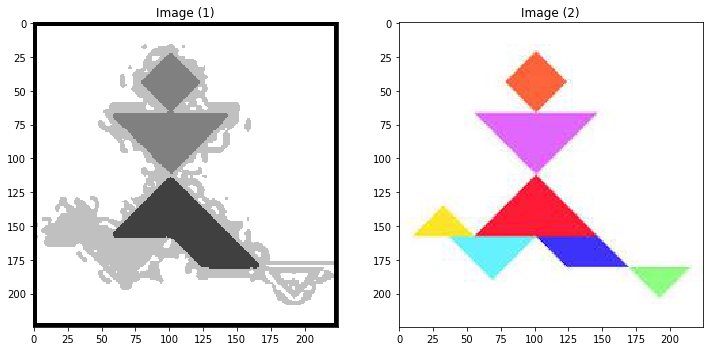
\includegraphics[width=.95\linewidth]{person_result.png}
        \\[\baselineskip]% adds vertical line spacing
        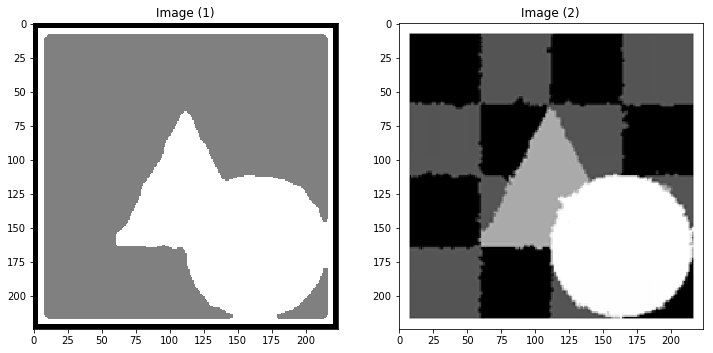
\includegraphics[width=.95\linewidth]{circle_result.png}
        %\\[\baselineskip]% adds vertical line spacing
        \caption{EM Segmentation with four/two classes of label on the left, original pictures on the right}
    \end{subfigure}
    ~
    \begin{subfigure}[b]{0.45\textwidth}
        \centering
        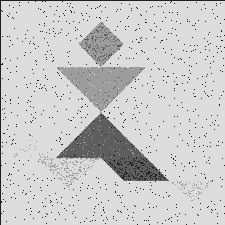
\includegraphics[width=.45\linewidth]{tangram_10.jpg}
        \\[\baselineskip]% adds ertical line spacing
        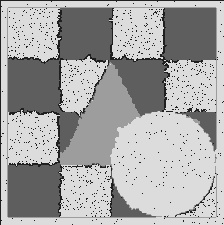
\includegraphics[width=.45\linewidth]{chess_circle_triangle_10.jpg}
        %\\[\baselineskip]% adds vertical line spacing
        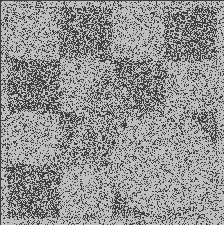
\includegraphics[width=.45\linewidth]{chess_circle_triangle_2_14.jpg}
        %\\[\baselineskip]% adds vertical line spacing
        \caption{Tabu search algorithm: first image is 10 iterations of the algorithm and 4 classes of labels. Left image on lower part is 10 iterations of the algorithm and 4 classes. The right image on lower part is 14 iterations of algorithm and 2 classes.}
    \end{subfigure}
%\end{center}
\caption{Algorithms results}
\label{fig:resultsAlgorithms}
\end{figure*}


The result of the EM algorithm is given in the figure above. The advantage of EM algorithm is that it always converges to a local minimum. So the stability of the algorithm is guaranteed. But in order to have a strictly convex problem at "M" step in each iteration, the potential function must not be parametrized. So the regularization prior needs to be fine-tuned for different images.

The result shows that EM does not perform well on relative complex images because it lacks the capacity to adapt the prior of the image throughout the training.

Another drawback effect of the EM algorithm can be seen in the second picture of Figure~\ref{fig:resultsAlgorithms}. There are some artifacts around the boundary of the person. Our explaination is that MRF only looks locally around each pixel. So there could be a "train-effects" of the labelling. The artifacts is caused by the similarity between the light color and the background color, and the error is propagate along the boundary.

\section{Conclusion}
We implemented/modified the MRF approach on image segmentation. We tried two different methods to solve the non-convex optimization problem. EM algorithm is more stable but is also constrained. Hybrid Tabu Search is more flexible in the sense that we don't follow any explicit assumption on the parameter space, but the algorithm takes quite a long time to run and works right now only for gray scale images, not colored images. Given our experimental results, some areas to improve the work are in the efficiency of the Tabu search method, the adaptation of the prior of the image in the EM algorithm and the extension of the MRF Tabu search method to use colored images. Regardless of these drawbacks, we think the algorithms based on MRF have potential to improve in the segmentation problem. Particularly, we think it would be very interesting to explore the interaction between deep learning and Markov Random Field techniques. 


\vskip 0.2in
\bibliography{reference}

% Manual newpage inserted to improve layout of sample file - not
% needed in general before appendices/bibliography.
%
%\newpage
%
%\appendix
%\section{}

\end{document}